\appendix

\chapter{Heat transfer under constant temperature}
Assuming $U$, $T_{c}$, $q_{m}$,$c_{p}$ to be constant, for given $T_{i}$,
\nomenclature[S]{$i$}{Inlet}

\noindent \begin{center}
\begin{figure}[h]
\begin{centering}
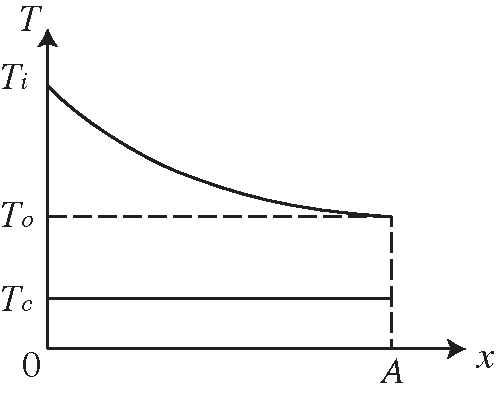
\includegraphics[width=0.6\textwidth]{fig/ConstTempHX.pdf}
\par\end{centering}
\caption{\label{fig:CTHX}Diagram of heat transfer under constant temperature}
\end{figure}
\par\end{center}

For $A(x)=Px$, $x$ from $0$ to $L$, while $T(x)$ from $T_{i}$ to $T_{o}$,
\nomenclature[S]{$o$}{Outlet}

\begin{equation}
q_{m}c_{p}dT(x)=(T_{c}-T(x))UPdx
\end{equation}

so

\begin{equation}
\frac{dT(x)}{dx}=-\frac{UP}{q_{m}c_{p}}(T(x)-T_{c})
\end{equation}

\begin{equation}
T_{g}(x)=T_{p}(x)+T_{h}(x)
\end{equation}

where $T_{g}(x)$ is the general solution, $T_{p}(x)$ is the particular
solution, $T_{h}(x)$ is the homogeneous solution.

\begin{equation}
-\frac{UP}{q_{m}c_{p}}(T_{p}(x)-T_{c})=0
\end{equation}

\begin{equation}
T_{p}(x)=T_{c}
\end{equation}

\begin{equation}
\frac{dT_{h}(x)}{dx}=-\frac{UP}{q_{m}c_{p}}T_{h}(x)\label{eq:T_h(x)}
\end{equation}

\begin{equation}
\int_{T_{h}(x)=T_{h}(0)}^{T_{h}(x)=T_{h}(L)}\frac{dT_{h}(x)}{T_{h}(x)}=-\int_{x=0}^{x=L}\frac{UP}{q_{m}c_{p}}dx
\end{equation}
\begin{equation}
\frac{T_{h}(L)}{T_{h}(0)}=\exp(-\frac{UPL}{q_{m}c_{p}})
\end{equation}

that is

\begin{equation}
\frac{T_{g}(L)-T_{p}(L)}{T_{g}(0)-T_{p}(0)}=\exp(-\frac{UA}{q_{m}c_{p}})
\end{equation}

\begin{equation}
\frac{T_{o}-T_{c}}{T_{i}-T_{c}}=\exp(-\frac{UA}{q_{m}c_{p}})
\label{eq:Eq}
\end{equation}

\chapter{Thermal gradient under constant heat flux}\label{cha:CTCHFHX}

Assuming $U$, $T_{c}$, $\dot{m}$, $c_p$, $q''$ to be constant, for
given $T_{i}$,

\noindent \begin{center}
\begin{figure}[h]
\noindent \begin{centering}
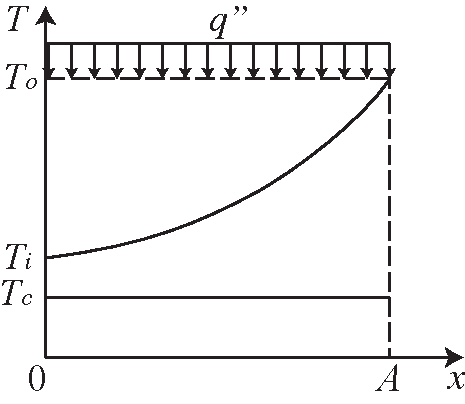
\includegraphics[width=0.6\textwidth]{fig/CTCHFHX.pdf}\caption{\label{fig:CTCHFHX}Diagram of heat transfer with one constant temperature
heat source and constant heat flux}
\par\end{centering}
\end{figure}
\par\end{center}

For $A(x)=Px$, $x$ from $0$ to $L$, while $T(x)$ from $T_{i}$ to $T_{o}$,
\begin{equation}
q_{m}c_{p}dT(x)=(T_{c}-T(x))UPdx+q''Pdx
\end{equation}

so

\begin{equation}
\frac{dT(x)}{dx}=-\frac{UP}{q_{m}c_{p}}T(x)+\frac{q''P+UPT_{c}}{q_{m}c_{p}}
\end{equation}
\nomenclature[S]{$g$}{General solution}\nomenclature[S]{$p$}{Particular solution}\nomenclature[S]{$h$}{Homogeneous solution}
\begin{equation}
T_{g}(x)=T_{p}(x)+T_{h}(x)
\end{equation}

where $T_{g}(x)$ is the general solution, $T_{p}(x)$ is the particular
solution, $T_{h}(x)$ is the homogeneous solution.

\begin{equation}
-\frac{UP}{q_{m}c_{p}}T_{p}(x)+\frac{q''P+UPT_{c}}{q_{m}c_{p}}=0
\end{equation}

\begin{equation}
T_{p}(x)=T_{c}+\frac{q''}{U}
\end{equation}

\begin{equation}
\frac{dT_{h}(x)}{dx}=-\frac{UP}{q_{m}c_{p}}T_{h}(x)
\end{equation}

the same as Equation (\ref{eq:T_h(x)}), so we have
\begin{equation}
\frac{T_{g}(L)-T_{p}(L)}{T_{g}(0)-T_{p}(0)}=\exp(-\frac{UA}{q_{m}c_{p}})
\end{equation}

\begin{equation}
\frac{T_{o}-T_{c}-\frac{q''}{U}}{T_{i}-T_{c}-\frac{q''}{U}}=\exp(-\frac{UA}{q_{m}c_{p}})
\end{equation}

%\chapter{Stirling engine model}\label{sec:Stirling-engine-model}
%
%A simple Stirling engine model is used for the system. The cycle efficiency is given by \cite{Stine1985}
%
%\begin{equation}
%	\eta=\frac{T_{H}-T_{L}}{T_{H}+\text{\ensuremath{\dfrac{1-e}{k-1}}}\cdot\dfrac{T_{H}-T_{L}}{\ln\gamma}}\label{eq:eta_stirling}
%\end{equation}
%
%
%where \nomenclature{$e$}{Regeneration effectiveness of the Stirling engine}$e = (T_{R}-T_{L}) / (T_{H}-T_{L})$,\nomenclature{$T_R$}{Regenerator temperature, K}$T_{R}$ is the\emph{ }regenerator temperature, \nomenclature{$c_p$}{Heat capacity of Stirling engine working gas at constant pressure, J/(kg$\cdot$K)}\nomenclature{$c_v$}{Heat capacity of Stirling engine working gas at constant volume, J/(kg$\cdot$K)}$k=c_{p}/c_{v}$ for the working gas, $\gamma_{se}=V_{max}/V_{min}$ is the compression ratio.
%
%The heat transfer diagram is shown in Figure~\ref{fig:Heat-transfer-diagram}. Flow 1 is used for heating the hot chamber of Stirling engine, $T_{1i}$ is the inlet temperature, $T_{1o}$ is the outlet temperature. Flow 2 is used for cooling the cold chamber of Stirling engine, $T_{2i}$ is the inlet temperature, $T_{2o}$ is the outlet temperature. \nomenclature{$T_H$}{Highest temperature of expansion space, K}$T_{H}$ is the highest temperature of expansion space, \nomenclature{$T_L$}{Lowest temperature of compression space, K}$T_{L}$ is the lowest temperature of compression space.
%
%\noindent \begin{center}
%\begin{figure}[h]
%	\noindent \centering{}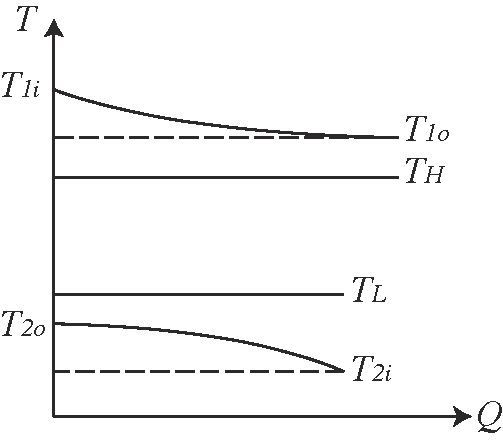
\includegraphics[width=0.4\columnwidth]{fig/StirilingHT}
%	\protect\caption{\label{fig:Heat-transfer-diagram}Heat transfer diagram of Stirling
%engine}
%\end{figure}
%
%\par\end{center}
%
%According to Equation (\ref{eq:Eq}),
%
%\begin{equation}
%	\dfrac{T_{1o}-T_{H}}{T_{1i}-T_{H}}=\exp(-\dfrac{U_{1}A_{1}}{\dot{m}_{1}c{}_{p1}})
%\end{equation}
%
%and
%
%\begin{equation}
%	\dfrac{T_{2o}-T_{L}}{T_{2i}-T_{L}}=\exp(-\dfrac{U_{2}A_{2}}{\dot{m}_{2}c_{p2}})
%\end{equation}
%
%So known $T_{1o},T_{1i},U_{1},A_{1},\dot{m}_{1},c_{p1},T_{2o},T_{2i},U_{2},A_{2},\dot{m}_{2},c_{p2}$, $T_{H}$ and $T_{L}$ can be calculated, and then $\eta$ can be obtained by using Equation (\ref{eq:eta_stirling}).
%\nomenclature{$A$}{Area, m$^2$}
  
\begin{publications}
  \item Zhang Cheng, Kun Wang. International Conference on Power Engineering: ICOPE 2013: FEA simulation on the alignment of the shafts of three-fulcrum turbine.
  \item Performance comparison of new and traditional arrangements of a dish-Stirling system
	\item A multi-stage exergy-loss reduction system for solar parabolic trough power plants
	\item Zhang Cheng, Zhang Yanping, Arauzo Inmaculada, Gao Wei, Zou Chongzhe. Cascade system using both trough system and dish system for power generation. Energy Convers Manag 2017;142:494–503. doi:10.1016/j.enconman.2017.03.073.
  \item Thermal Modeling of a Pressurized Air Cavity Receiver for a Solar Dish Stirling System
  
  \item A solar thermal cascade system, No. 201610806296.5
  \item A flow control method used in a multi-stage heating system, No. 201610805604.2
  
\end{publications}